Part of speech tagging is one the most important NLP tasks. The
task is to assign each word a grammatical category, \emph{i.e.} Noun,
Verb, Adjective, ... . In English, using the Penn Treebank (PTB)~\citep{pennTreeBank}, the current
state of the art for part of speech tagging is around 97\% for a
variety of methods \footnote{See ACL state of the art wiki}.

In the rest of this class we will use a subset of the PTB corpus, but
instead of using the original 45 tags we will use a reduced tag set of
12 tags, to make the algorithms faster for the
class. In this task, $x$ is a sentence (\emph{i.e.}, a sequence of word tokens) and $y$
is the sequence of possible PoS tags.

The first step is to load the corpus. We will start by loading
1000 sentences for training and 200 sentences both for development and
testing. Then we train the HMM model by maximum 
likelihood estimation.
\begin{python}
>>> import readers.pos_corpus as pcc
>>> corpus = pcc.PostagCorpus()
>>> train_seq = corpus.read_sequence_list_conll("../data/train-02-21.conll",max_sent_len=15,max_nr_sent=1000)
unknown tag po
unknown tag pr
unknown tag wd
unknown tag pd
unknown tag wr
unknown tag sy
>>> test_seq = corpus.read_sequence_list_conll("../data/test-23.conll",max_sent_len=15,max_nr_sent=1000)
unknown tag pr
unknown tag po
unknown tag wr
unknown tag wd
unknown tag pd
unknown tag sy
>>> dev_seq = corpus.read_sequence_list_conll("../data/dev-22.conll",max_sent_len=15,max_nr_sent=1000)
unknown tag wd
unknown tag wr
unknown tag po
unknown tag pr
unknown tag pd
>>> hmm = hmmc.HMM(corpus.word_dict, corpus.tag_dict)
>>> hmm.train_supervised(train_seq)
>>> hmm.print_transition_matrix()
\end{python}

Ignore the warnings -- they are a consequence of our choice of using only a reduced set of 12 tags instead of the full set of POS tags.

%Note the warning ``Warning: invalid value encountered in divide`` due to the lack of smoothing. This is because we are trying to
%estimate the probability of words that were never seen during
%training, so the counts are zero and, when normalizing to get probabilities, we are trying to do 0/0. 

Look at the transition probabilities of the trained model
%\begin{python}
%In []: import matplotlib.pyplot as plt
%In []: hmm.transition_probs
%\end{python}
 (see
Figure \ref{fig:transProbs}), and see if they match your intuition
about the English language (e.g. adjectives tend to come before nouns).

\begin{figure}
\centering
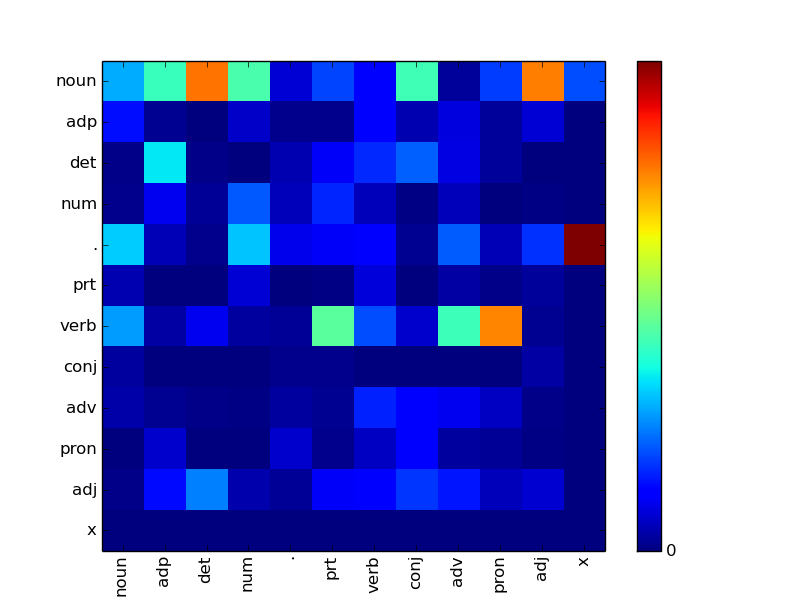
\includegraphics[scale=.5]{figs/sequences/transition_probs}
\caption{\label{fig:transProbs} Transition probabilities of the
trained model. Each column is previous state and row is current
state. Note the high probability of having Noun after Adjective, or of having Verb after Noun, as expected.}
\end{figure}

\begin{exercise}
Test the model using both posterior decoding and Viterbi decoding on
both the train and test set, using the methods in class HMM:
\begin{python}
>>> viterbi_pred_train = hmm.viterbi_decode_corpus(train_seq)
>>> posterior_pred_train = hmm.posterior_decode_corpus(train_seq)
>>> eval_viterbi_train =   hmm.evaluate_corpus(train_seq, viterbi_pred_train)
>>> eval_posterior_train =  hmm.evaluate_corpus(train_seq, posterior_pred_train)
>>> print "Train Set Accuracy: Posterior Decode \%.3f, Viterbi Decode: \%.3f"\%(eval_posterior_train,eval_viterbi_train)
Train Set Accuracy: Posterior Decode 0.981, Viterbi Decode: 0.981
>>> viterbi_pred_test = hmm.viterbi_decode_corpus(test_seq)
>>> posterior_pred_test = hmm.posterior_decode_corpus(test_seq)
>>> eval_viterbi_test =   hmm.evaluate_corpus(test_seq,viterbi_pred_test)
>>> eval_posterior_test = hmm.evaluate_corpus(test_seq,posterior_pred_test)
>>> print "Test Set Accuracy: Posterior Decode \%.3f, Viterbi Decode: \%.3f"\%(eval_posterior_test,eval_viterbi_test)
Test Set Accuracy: Posterior Decode 0.380, Viterbi Decode: 0.522
\end{python}

What do you observe? Remake the previous exercise but now train the HMM
using smoothing. Try different values (0,0.1,0.01,1) and report the results on the
train and development set. (Use function
\emph{pick\_best\_smoothing}).


\begin{python}
>>> best_smothing = hmm.pick_best_smoothing(train_seq, dev_seq, [10,1,0.1,0])
>>> hmm.train_supervised(train_seq, smoothing=best_smothing)
>>> viterbi_pred_test = hmm.viterbi_decode_corpus(test_seq)
>>> posterior_pred_test = hmm.posterior_decode_corpus(test_seq)
>>> eval_viterbi_test =   hmm.evaluate_corpus(test_seq, viterbi_pred_test)
>>> eval_posterior_test = hmm.evaluate_corpus(test_seq, posterior_pred_test)
>>> print "Best Smoothing \%f --  Test Set Accuracy: Posterior Decode \%.3f, Viterbi Decode: \%.3f"%(best_smothing,eval_posterior_test,eval_viterbi_test)
Best Smoothing 0.100000 --  Test Set Accuracy: Posterior Decode 0.855, Viterbi Decode: 0.838
\end{python}

%As before, the warnings are due to tags in the dev set which were not present in the train set -- just ignore them. Using the best smoothing value (0.1) evaluate the accuracy on the test set.
%
%\begin{python}
%In []: hmm.train_supervised(train_seq,smoothing=0.1)
%In []: pred = hmm.viterbi_decode_corpus(test_seq.seq_list)
%In []: eval_test = hmm.evaluate_corpus(test_seq.seq_list,pred)
%In []: eval_test
%Out[]: 0.8377896613190731
%\end{python}

Perform some error analysis to understand were the errors are coming
from. You can start by visualizing the confusion matrix (true tags vs
predicted tags). You should get something like \ref{fig:cm_uns}.

\begin{python}
>>> import sequences.confusion_matrix as cm
>>> confusion_matrix = cm.build_confusion_matrix(test_seq.seq_list, viterbi_pred_test, len(corpus.tag_dict), hmm.get_num_states())
>>> cm.plot_confusion_bar_graph(confusion_matrix, corpus.tag_dict, xrange(hmm.get_num_states()), 'Confusion matrix')
>>> plt.show()
\end{python}

\begin{figure}
\centering
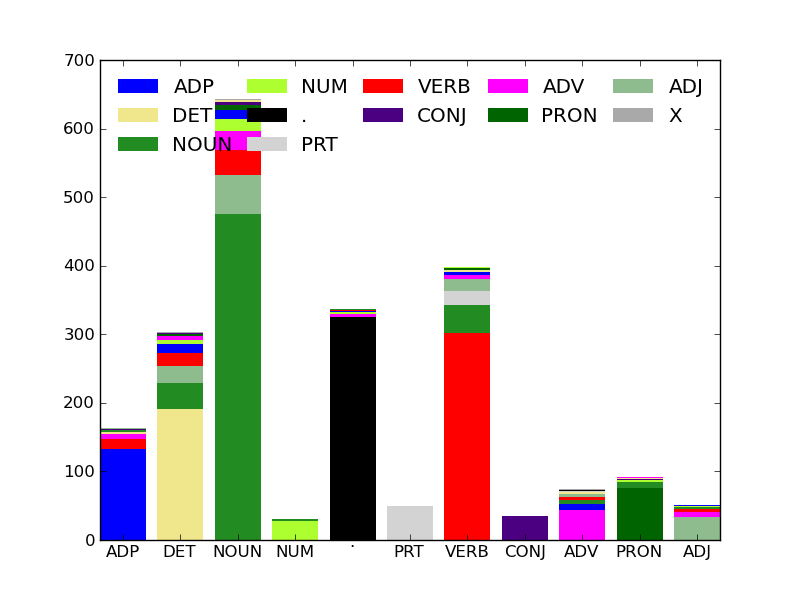
\includegraphics[scale=.5]{figs/sequences/cm_sup.png}
\caption{\label{fig:cm_uns} Confusion Matrix for the previous
  example. Predict tags are columns and the true tags corresponds to
  the constituents of each column.}
\end{figure}

%Another option to look at is to the error for words with different
%number of occurrences, rare words vs common words.
\end{exercise}


%\begin{exercise}
%Implement a function that produces the accuracy for rare words vs
%common words. Use you own definition of rare word.
%
%Can you come up with other error analysis methods? Which?
%
%\end{exercise}

%\begin{exercise}
%So far we have only worked with a limited dataset of 1000 words. Try increasing the number of sentences to 10000. What do you observe?
%\end{exercise}


\section{Unsupervised Learning of HMMs}

\afm{explain here the EM algorithm}

\begin{python}
>>> hmm.train_EM(train_seq, best_smothing, 20, evaluate=True)
Initial accuracy: 0.368073
Iter: 1 Log Likelihood: -101710.745014
Iter: 1 Accuracy: 0.397134
Iter: 2 Log Likelihood: -78077.788430
Iter: 2 Accuracy: 0.417276
Iter: 3 Log Likelihood: -77903.286662
Iter: 3 Accuracy: 0.431105
Iter: 4 Log Likelihood: -77439.879115
Iter: 4 Accuracy: 0.427197
Iter: 5 Log Likelihood: -76472.011310
Iter: 5 Accuracy: 0.427899
Iter: 6 Log Likelihood: -74985.839947
Iter: 6 Accuracy: 0.427197
Iter: 7 Log Likelihood: -73145.793548
Iter: 7 Accuracy: 0.427197
Iter: 8 Log Likelihood: -71327.155828
Iter: 8 Accuracy: 0.422688
Iter: 9 Log Likelihood: -69754.925747
Iter: 9 Accuracy: 0.422187
Iter: 10 Log Likelihood: -68439.400115
Iter: 10 Accuracy: 0.421485
Iter: 11 Log Likelihood: -67367.537999
Iter: 11 Accuracy: 0.421485
Iter: 12 Log Likelihood: -66503.458319
Iter: 12 Accuracy: 0.421385
Iter: 13 Log Likelihood: -65961.609556
Iter: 13 Accuracy: 0.421385
Iter: 14 Log Likelihood: -65734.329382
Iter: 14 Accuracy: 0.421285
Iter: 15 Log Likelihood: -65650.388117
Iter: 15 Accuracy: 0.421285
Iter: 16 Log Likelihood: -65618.797337
Iter: 16 Accuracy: 0.421285
Iter: 17 Log Likelihood: -65606.269066
Iter: 17 Accuracy: 0.421285
Iter: 18 Log Likelihood: -65600.359979
Iter: 18 Accuracy: 0.421285
Iter: 19 Log Likelihood: -65596.566323
Iter: 19 Accuracy: 0.421385
>>> confusion_matrix = cm.build_confusion_matrix(test_seq.seq_list, viterbi_pred_test, len(corpus.tag_dict), hmm.get_num_states())
>>> cm.plot_confusion_bar_graph(confusion_matrix, corpus.tag_dict, xrange(hmm.get_num_states()), 'Confusion matrix')
\end{python}